\documentclass{article}
\usepackage{graphicx} % Required for inserting images
\usepackage{tikz}
\usepackage[landscape]{geometry}
\usepackage{float}
\usepackage{listings}

%arrange page numbers
\usepackage{fancyhdr}
\pagestyle{fancy}
\fancyhf{}
\renewcommand{\headrulewidth}{0pt}
\fancyhead[R]{\thepage}

%setup Tikz to draw the graphs
\usetikzlibrary{external}
\tikzexternalize 
%load options
\usetikzlibrary{positioning, calc, shapes.geometric, shapes.multipart,
        shapes, arrows.meta, arrows, decorations.markings, external, trees}

%Create custom arrow style:
\tikzstyle{Arrow} = [
thick,
decoration={
markings,
mark=at position 0.9999 with {
\arrow[thick]{latex}}},
shorten >= 3pt, preaction = {decorate}]



\title{Box DAGs}
\author{tpfeeney }
\date{June 2023}

\begin{document}

\section{Box DAG}
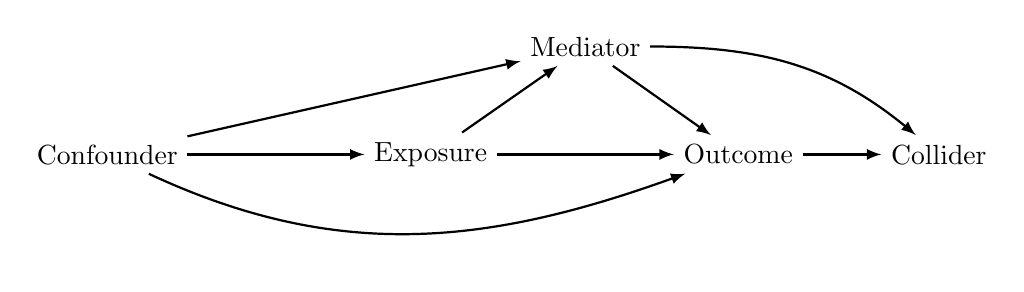
\begin{tikzpicture}
    \node (1) {};
    \node [right =of 1] (2)  {Exposure};
    \node [right =of 2] (3) {};
    \node [right =of 3] (4) {Outcome};
    \node [left =of 1] (5) {Confounder};
    \node [above =of 3] (6) {Mediator};
    \node [right =of 4] (7) {Collider};

    \draw[Arrow] (2.east)--(4.west);
    \draw[Arrow] (2) to (6);
    \draw[Arrow] (6) to (4);
    \draw[Arrow] (5) to [out=-25, in=-160](4);
    \draw[Arrow] (5) to (6);
    \draw[Arrow] (5.east)--(2.west);
    \draw[Arrow] (4.east)--(7.west);
    \draw[Arrow] (6) to [out=0, in=140] (7);
\end{tikzpicture}

\subsection*{node}

\subsection*{edge}
\begin{tikzpicture}
    \node (1) {};
    \node [right =of 1] (2) {};
    \draw[Arrow] (1) to (2);
\end{tikzpicture}
    
\subsection*{confounder}

\begin{tikzpicture}
    \node (1) {confounder};
    \node [right =of 1] (2) {exposure};
    \node [right =of 2] (3) {outcome};
    \draw [Arrow] (1) to (2);
    \draw [Arrow] (1) to [out=20, in=160] (3);
\end{tikzpicture}

\subsection*{mediator; indirect effects}
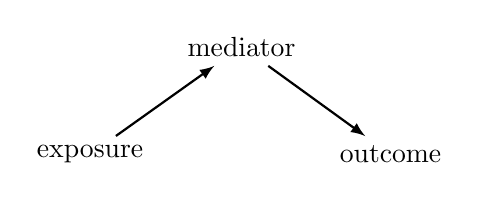
\begin{tikzpicture}
    \node (1) {exposure};
    \node [right =of 1] (2) {};
    \node [right =of 2] (3) {outcome};
    \node [above =of 2] (4) {mediator};
    \draw [Arrow] (1) to (4);
    \draw [Arrow] (4) to (3);
\end{tikzpicture}

\subsection*{direct effects}

\begin{tikzpicture}
    \node (1) {exposure};
    \node [right =of 1] (3) {outcome};
    \draw [Arrow] (1) to (3);
\end{tikzpicture}

\subsection*{collider}
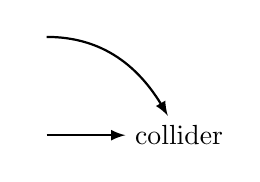
\begin{tikzpicture}
    \node (1) {};
    \node [right =of 1] (2) {collider};
    \node [above =of 1] (3) {};
    \draw [Arrow] (1) to (2);
    \draw [Arrow] (3) to [out=0, in=120] (2);
\end{tikzpicture}

\end{document}
